\chapter{Simplified Tools}

\label{Simp:Tool:One}


This chapter describes simplified tools that allow to make
computations without filling XML-files.
Of course they cannot deal with all the situation that are
handled by complex tools, but I hope that in near future they
will be sufficient for $95\%$ of usages.


\section{All in one command}

Sorry this tool does not exist, but it will come \dots

%-------------------------------------------------------------------
%-------------------------------------------------------------------
%-----------------------------------------------------------------




\section{Computing Tie Points with Tapioca}

{\tt Tapioca} is a simple tool interface for computing tie points.
I think {\tt Tapioca}  should be sufficient in $95\%$ of cases.
If it is not the case, you will have to refer to a more complex and powerful
tool named {\tt Pastis} which will be described later.
In fact, {\tt Tapioca} is only an interface to {\tt Pastis}
\footnote{{\tt Pastis}  being itself an interface to \SiftPP \dots}.

\label{Tapioca}

    % - - - - - - - - - - - - - - - - - - - - -

\subsection{General Structure}

If {\tt bin/Tapioca} does not exit, build it with {\tt make bin/Tapioca}.

The general syntax of {\tt Tapioca} is:

\begin{center}
   {\tt bin/Tapioca   Mode  Files  Arg1 Arg2  \dots Opt1=Val Opt2=Val \dots}
\end{center}

Here are possible \UNCLEAR{use} of {\tt Tapioca}:

{\scriptsize
\begin{verbatim}
bin/Tapioca All  "../micmac_data/ExempleDoc/Boudha/IMG_[0-9]{4}.tif" -1  ExpTxt=1
bin/Tapioca Line  "../micmac_data/ExempleDoc/Boudha/IMG_[0-9]{4}.tif" -1   3 ExpTxt=1
bin/Tapioca MulScale "../micmac_data/ExempleDoc/Boudha/IMG_[0-9]{4}.tif" 300 -1 ExpTxt=1
bin/Tapioca File  "../micmac_data/ExempleDoc/Boudha/MesCouples.xml" -1  ExpTxt=1
\end{verbatim}
}


The meaning of arguments is:

\begin{itemize}

    \item {\tt Mode} is an enumerated value specifying a functioning mode
          (i.e. a way to compute the pair of images that are to be matched).
          These values are {\tt All} for all possible pairs, {\tt MulScale}
          for a multi-scale optimization, {\tt Line} for a selection adapted 
          to linear images acquisition, and {\tt File} for  XML file
          describing the pairs;

    \item {\tt Files} specifies a set of images to be matched. For all these
         images, a set of sift descriptor will be computed. However, all the pairs of
         descriptors sets will not be  matched. To optimize the computation, a subset
         of \UNCLEAR{images pair} will be described by the {\tt Mode} parameters.
         The first part of {\tt Files} is a directory, and the second one is the description
         of the files to be computed with Tapioca.
         The results will be written in the subdirectory {\tt Homol} of the
         specified directory as it was described in~\ref{Tie:Poi:Ex:Apero};



    \item  {\tt Arg1 Arg2  \dots} are mandatory parameters; their number depends
           upon {\tt Mode}, it always includes a resolution parameter;

    \item  {\tt  Opt1=Val Opt2=Val  \dots} are optional parameters. The possible
           optional parameters depends upon {\tt Mode}.
           There is always at least two possible optional parameters:

            \begin{itemize}
                 \item {\tt ExpTxt} indicates if you want an export in text mode;
                       default is $0$ (binary mode);

                 \item {\tt ByP} indicates the number of processors that will be used
                        to \UNCLEAR{parallelize the process}; %simultaneously
                       default is the number of
                        processors described in~\ref{Mic:File:Config}.
            \end{itemize}

\end{itemize}

If you do not remember the possible mode key words, just type: 

\begin{center}
        {\tt bin/Tapioca}
\end{center}

The possible values will be printed. 

If you do not remember the argument 
corresponding to a possible mode, just type {\tt bin/Tapioca mode -help},
for example:

\begin{center}
        {\tt bin/Tapioca MulScale -help}
\end{center}



    % - - - - - - - - - - - - - - - - - - - - -

\subsection{Computing All the Tie Points of a Set of Images}

The simplest case of use of {\tt Tapioca} is when you only want to compute tie points
between all the pairs of a set of images. The syntax is: 

{\scriptsize
\begin{verbatim}
    bin/Tapioca All  Files  Size  ArgOpt=
\end{verbatim}
}

The only optional arguments are those common to all modes ({\tt ExpTxt}  and {\tt ByP}).

The parameter {\tt Files} is the concatenation of the directory where the files
are located with a regular expression used as a filter on the existing files
of the directory.

The parameter {\tt Size} is used to shrink the images. It does not specify
a scale but the desired width for shrinking the images. For example, if the initial
image has a width of $5000$, and the value is $2000$, it will specify
a scaling of $0.4$. If its value is $-1$, it means, conventionally, no shrinking.
This is the value chosen in the examples, in order  to limit the size of the transmitted
data, the images have already been shrinked. With real images, I do not
recommend the value $-1$ but rather a value corresponding to a scaling
between $0.3$ and $0.5$.


The example:

{\scriptsize
\begin{verbatim}
    bin/Tapioca All  "../micmac_data/ExempleDoc/Boudha/IMG_[0-9]{4}.tif" -1  ExpTxt=1
\end{verbatim}
}

It generates tie points computation between all the pairs of images of the {\tt Boudha} directory,
with names matching {\tt IMG\_[0-9]{4}.tif}. There is no shrinking, the export is
made in text mode.

    % - - - - - - - - - - - - - - - - - - - - -

\subsection{Optimization for Linear Canvas}

It often occurs that the photos canvas  has a linear structure, for example, when you acquire
photos of a facade walking  along the street.   In thise case, you
know that $K^{th}$  can only have tie points
with images in the interval $[K-\delta,K+\delta]$; giving this information
to Tapioca can save a lot of time. The syntax is:

{\scriptsize
\begin{verbatim}
    bin/Tapioca Line  Files  Size  delta ArgOpt=
\end{verbatim}
}

{\tt delta} is $\delta$ and all the other arguments have the same meaning as in the
 {\tt All} mode.

    % - - - - - - - - - - - - - - - - - - - - -

\subsection{Multi Scale Approach}


The mode  {\tt MulScale} can save  significant computation time on large sets of images.
Even if it is not optimal for all canvas, it has the benefit of being general
and usable with any data set.

In this mode, a first computation of tie points is made for all the pairs 
of images at very low resolution (so it is quite fast).Then the 
computation, at the desired resolution, is done  only for the pairs
having, at low resolution, a number  of tie points exceding a given
threshold.



{\scriptsize
\begin{verbatim}
     bin/Tapioca MulScale Files  SizeLow Size  NbMinPt=   ArgOpt=
\end{verbatim}
}
 
{\tt SizeLow} is the size of the images that will be used at low resolution.
{\tt Size} is the targeted size.  The optional value {\tt NbMinPt}
is the threshold on the number of tie points detected at low resolution,
its default value is $2$. For example:

{\scriptsize
\begin{verbatim}
    bin/Tapioca MulScale "../micmac_data/ExempleDoc/Boudha/IMG_[0-9]{4}.tif" 300 -1 ExpTxt=1
\end{verbatim}
}

Computes  tie points with images of width of $300$, and if the pairs have at least
$2$ tie points, it does the computation at full resolution.


    % - - - - - - - - - - - - - - - - - - - - -

\subsection{Explicit Specification of images pairs} %of the Pairs of Images

Sometimes, you will have external information (like embedded GPS) that allows
you to know which pairs of images are potential candidates for tie points.
If you are familiar with computer programming, you will find that
the easiest way to communicate your information is to write a file
containing the explicit list of pairs of images.
It is possible in the {\tt File} mode, the file containing
the pairs must have the following structure:

{\scriptsize
\begin{verbatim}
<?xml version="1.0" ?>
<SauvegardeNamedRel>
     <Cple>IMG_5564.tif IMG_5565.tif</Cple>
     <Cple>IMG_5574.tif IMG_5575.tif</Cple>
     <Cple>IMG_5580.tif IMG_5579.tif</Cple>
     <Cple>IMG_5581.tif IMG_5582.tif</Cple>
</SauvegardeNamedRel>
\end{verbatim}
}

The syntax is:


{\scriptsize
\begin{verbatim}
    bin/Tapioca File  NameOfFile  Size   ArgOpt=
\end{verbatim}
}

The pairs contained in the file {\tt NameOfFile} are names relative
to the directory indicated by the first part of {\tt NameOfFile}.
For example in:

{\scriptsize
\begin{verbatim}
bin/Tapioca File  "../micmac_data/ExempleDoc/Boudha/MesCouples.xml" -1  ExpTxt=1
\end{verbatim}
}


In the pair {\tt <Cple>IMG\_5564.tif IMG\_5565.tif</Cple>}, the first name means
\newline
{\tt "../micmac\_data/ExempleDoc/Boudha/IMG\_5564.tif}.




\subsection{The tool {\tt GrapheHom}}

A tool for generating a file image pairs, as input to {\tt Tapioca File \dots } from external Data (GPS or GPS-INS).

\begin{verbatim}
GrapheHom  -help
*****************************
*  Help for Elise Arg main  *
*****************************
Unamed args : 
  * string
  * string
  * string
Named args : 
  * [Name=TagC] string
  * [Name=TagOri] string
  * [Name=AltiSol] REAL
  * [Name=Dist] REAL
  * [Name=Rab] REAL
  * [Name=Terr] bool
  * [Name=Sym] bool
  * [Name=Out] string

\end{verbatim}

The three first mandatory args :

\begin{itemize}
   \item directory ;

   \item a pattern describing the set of images (it can also be a key of set);

   \item a key association for computing the name of the \emph{a priori }localisation file;
         this file must always contains  defining the image position of type {\tt Pt3dr}
         (by default in the tag {\tt Centre});
         optionnaly it can contains a tag  of type {\tt OrientationConique}  defining
         the approximative orientation (by default this tag is  {\tt OrientationConique});
\end{itemize}


The optional args :

\begin{itemize}
    \item {\tt \bf TagC} XML tag for centre (default = {\tt Centre});
    \item {\tt \bf TagOri} XML tag for orientation (default = {\tt OrientationConique});
    \item {\tt \bf AltiSol}  altitude of ground when it cannot be found in orientation files
           (default = $0.0$);
    \item {\tt \bf Terr}   is a terrestrial or aerial acquisition, (default = {\tt false}, i.e; aerial);
    \item {\tt \bf Dist}  minimal distance between two submit, optional in aerial mission
          (a default value will be computed) mandatory in terrestrial acquisition;
\end{itemize}


For example :

\begin{verbatim}
GrapheHom ./   ".*.ARW" NKS-Assoc-Im2Orient@-A0-Navig-UTM
Or 
GrapheHom ./   ".*.ARW" -A0-Navig-UTM
\end{verbatim}




%-------------------------------------------------------------------
%-------------------------------------------------------------------
%-------------------------------------------------------------------

\section{Simple relative orientation and calibration with Tapas}


     % - - - - - - - - - - - - - - - - -  - - - - - 

\subsection{Generalities}

The general tool for computing orientation of images is {\tt Apero},
this is a relatively complex tool an overview of which is given in chapter~\ref{Intro:QuickApero}.
These sections describe a set of basic tools offering a simplified interface
to some of the elementaries functionalities of {\tt Apero} :

\begin{itemize}
   \item {\tt Tapas}, in this section, is a tool offering most of the possibilities
         of {\tt Apero} for computing purely relative orientations;

   \item {\tt AperiCloud}, in~\ref{APERICLOUD} for generating a vizualisation of camera
         position and sparse $3D$ model;
		 
   \item {\tt Campari}, in~\ref{CAMPARI} is a tool for compensation of heterogenous measures (tie points and ground control points);

   \item {\tt Bascule}, in~\ref{BASCULE}, for generating orientations coherent with
        some physical information on the scene;

   \item {\tt MakeGrid}, in~\ref{MAKEGRID}, for generating   orientations  in a grid
         format that is more adapted to some further processing;

\end{itemize}

Like with many tools, one can type {\tt Tapas -help} to a have a brieve description
of {\tt Tapas}'s argument.

     % - - - - - - - - - - - - - - - - -  - - - - - 

\subsection{The data set  "Mur Saint Martin"}

        %  -    -    -    -    -    -    -     -


The directory {\tt MurSaintMartin/} in {\tt micmac\_data/ExempleDoc/}, contains 
a first set of data, that will be used for illustrating {\tt Tapas}.
This set is made of $23$ jpeg images that have been acquired with the same
camera and same focal length; it is made of two subset :

\begin{itemize}
    \item $17$ images of a wall : images {\tt IMGP4167.JPG} to {\tt IMGP4183.JPG}, the first
          $8$ images are presented on figure~\ref{FIG:StM:Mur};
    \item $6$ images of a corner, that can be optionnally used for intrinsic calibration
           : images {\tt IMGP4160.JPG} to {\tt IMGP4165.JPG}, the images are on figure~\ref{FIG:StM:Calib} ;
\end{itemize}



\begin{figure}
\begin{center}
\includegraphics[height=28mm]{FIGS/MurSaintMartin/Small-IMGP4167.JPG}
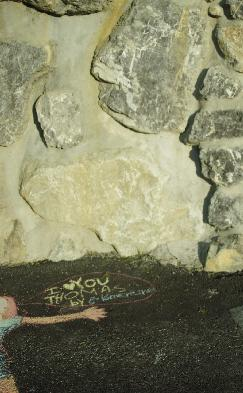
\includegraphics[height=28mm]{FIGS/MurSaintMartin/Small-IMGP4168.JPG}
\includegraphics[height=28mm]{FIGS/MurSaintMartin/Small-IMGP4169.JPG}
\includegraphics[height=28mm]{FIGS/MurSaintMartin/Small-IMGP4170.JPG}
\includegraphics[height=28mm]{FIGS/MurSaintMartin/Small-IMGP4171.JPG}
\includegraphics[height=28mm]{FIGS/MurSaintMartin/Small-IMGP4172.JPG}
\includegraphics[height=28mm]{FIGS/MurSaintMartin/Small-IMGP4173.JPG}
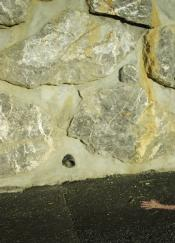
\includegraphics[height=28mm]{FIGS/MurSaintMartin/Small-IMGP4174.JPG}
\end{center}
\caption{The set of images of  Saint Martin, images of the wall}
\label{FIG:StM:Mur}
\end{figure}


\begin{figure}
\begin{center}
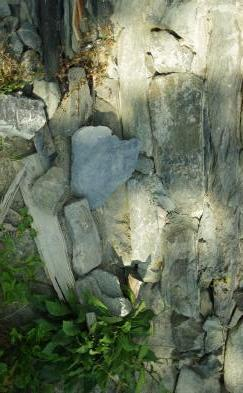
\includegraphics[width=25mm]{FIGS/MurSaintMartin/Small-IMGP4160.JPG}
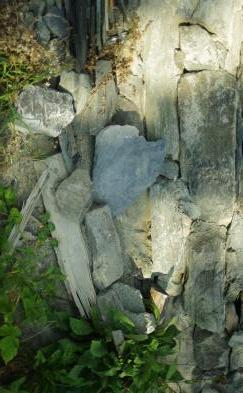
\includegraphics[width=25mm]{FIGS/MurSaintMartin/Small-IMGP4161.JPG}
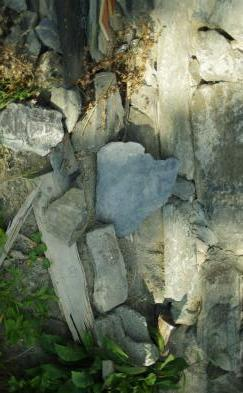
\includegraphics[width=25mm]{FIGS/MurSaintMartin/Small-IMGP4162.JPG}
\includegraphics[width=25mm]{FIGS/MurSaintMartin/Small-IMGP4163.JPG}
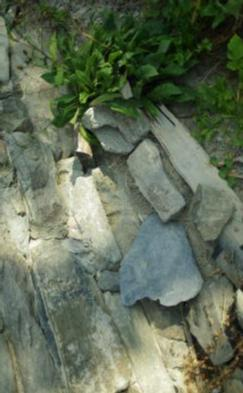
\includegraphics[width=25mm]{FIGS/MurSaintMartin/Small-IMGP4164.JPG}
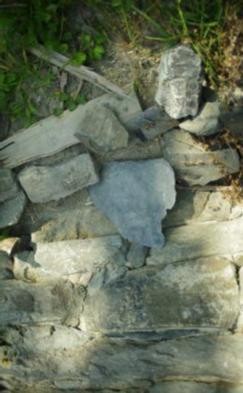
\includegraphics[width=25mm]{FIGS/MurSaintMartin/Small-IMGP4165.JPG}
\end{center}
\caption{The set of images of  Saint Martin, images for intrinsic calibration}
\label{FIG:StM:Calib}
\end{figure}

To run the example using {\tt Tapas}, tie points will be required, they can
be computed by the two  commands \footnote{the  command  used in this example can be found in  
the file {\tt ExCmd.txt}} :


\begin{verbatim}
Tapioca All "IMGP416[0-5].JPG" 1000
Tapioca Line "IMGP41((6[7-9])|([7-8][0-9])).JPG" 1000 4
\end{verbatim}

        %  -    -    -    -    -    -    -     -

\subsection{Basic usage}


\label{Basi:Tapas}

        %  -    -    -    -    -    -    -     -
\subsubsection{Syntax}

The basic command to run  {\tt Tapas} is :

\begin{center}
   {\tt Tapas  ModeCalib  PatternImage}
\end{center}

Where :

\begin{itemize}
    \item {\tt ModeCalib} is an enumerated value specifying a model
          of calibration;
    \item {\tt PatternImage} is a pattern specifying the subset of images
          to orientate;
\end{itemize}

For example the command :


\begin{verbatim}
Tapas RadialExtended "IMGP41((6[7-9])|([7-8][0-9])).JPG"
\end{verbatim}

Means :


\begin{itemize}
   \item compute the relative orientation of the set of images defined by the regular 
         expression ;

   \item for the intrinsic calibration use a model {\tt RadialExtended};

    \item there is exactly one intrinsic calibration unknown for each focal length, the focal
          length being extracted from exif metadata; the exif meta-data is used for 
          defining the  initial value of each 

    \item  use a predefined strategy for computing orientations and intrinsic calibration.
         
\end{itemize}

        %  -    -    -    -    -    -    -     -

\subsubsection{Distorsion models}
\label{Tap:Dis:Mod}

The possible value of  {\tt ModeCalib} are :


\begin{itemize}

   \item {\tt \bf RadialExtended} a model with radial distorsion 
         (as specified in~\ref{SpGeo:Rad}); 
         in this model there are $10$ degrees of freedom:
         $1$ for focal length  , $2$ for principal point, $2$ for distorsion center , 
         $5$ for coefficients of radial distorsion ($r^3$, $r^5$ \dots $r^{11}$);

   \item {\tt \bf RadialBasic}  a "subset" of previous model:
          radial distorsion with limited degrees of freedom ;
         adapted when there is a risk of divergence of {\tt RadialExtended}; 
         in this model there are $5$ degrees of freedom :  $1$ for focal length  , 
         $2$ for principal point and distorsion center \footnote{they are constrained to have 
         the same value} ,
         $2$ for coefficients of radial distorsion ($r^3$ and  $r^5$);



   \item {\tt \bf Fraser}  a radial model, with decentric and affine parameters
          (as specified in~\ref{SpGeo:Fraser}); there are $12$ degrees of freedom:
         $1$ for focal length  , $2$ for principal point, $2$ for distorsion center , 
         $3$ for coefficients of radial distorsion ($r^3$, $r^5$  $r^7$),
         $2$ for decentric parameters, $2$ for affine parameters;
         the optional parameters {\tt LibAff} and {\tt LibDec} (def value true) can
         be set to false if decentric of affine parameters must stay frozen;


   \item {\tt \bf FraserBasic}  same as previous with for principal point and distorsion center
         constrained to have the same value (so $10$ degree of freedom);

   \item {\tt \bf FishEyeEqui}  a model adapted for diagonal fisheyes equilinear
         ( with $atan$ physicall model completed with polynomial parameters,
          as specified in~\ref{SpGeo:FishEye}); there are $14$ degrees of freedom:
         $1$ for focal length  , $2$ for principal point, $2$ for distorsion center , 
         $5$ for coefficients of radial distorsion ($r^3$, $r^5$  $r^7$),
         $2$ for decentric parameters, $2$ for affine parameters;
         by default the ray defining the usefull masq, see~\ref{SpGep:RU}
         is $95\%$ of the diagonal;


   \item {\tt \bf HemiEqui}  same model as previous, but  by default the ray defining 
         the usefull masq, see~\ref{SpGep:RU} is $52\%$ of the diagonal; adapted
         to hemispherique equilinear fisheye;


   \item {\tt \bf AutoCal} and {\tt \bf Figee} , with this tag no model is defined,
         all the calibration must have a value (via {\tt InCal} or {\tt InOri} options);
         with {\tt  AutoCal} the calibration are re-evaluated while with {\tt  Figee}
         it stay frozen.

\end{itemize}


For all the mode, except of course {\bf AutoCal} and {\tt Figee},  the initial
value of intrinsic calibration is computed this way :

\begin{itemize}
   \item focal length is computed from exif data using the rules described in~\ref{CamDB};

   \item principal point and, when apply, distorsion centre are  at the middle 
         of image (except when using the {\tt Decentre} option);

   \item initial distorsion is equal to the physcical ideal model :   nul for the
         standar lenses and equal to $atant$ for  fisheye;

\end{itemize}

        %  -    -    -    -    -    -    -     -
\subsubsection{Strategy}

With {\tt Tapas}, the user has very few control on the  strategy used to compute
orientation.  The predefined strategy used by {\tt Tapas} is :

\begin{itemize}
   \item initialize all the intrinsic calibration using exif data (or already c
         computed calibration provided by existing files), then freeze all these unknown;

   \item choose a central images (the image that has the maximum of tie points);

   \item compute the orientation of images with the "standard" strategy described 
          in~\ref{Apero:Ordering};


   \item once all the image are ordered, free in a predifined order all the intrinsic
         parameters;

\end{itemize}

\subsubsection{Results}

The result of {\tt Tapas} are stored in a subdirectory {\tt Ori-OUTDIR} , 
where {\tt OUTDIR} is specified by the optional {\tt out} argument of {\tt Tapas},
when {\tt out} is not specified the value of {\tt ModeCalib} is used.
With this basic command, the result are stored in the directory {\tt Ori-RadialExtended/} :



\begin{itemize}
   \item the file {\tt AutoCal280.xml} contains the intrinsic calibration; the name
         has been automatically computed from the focal lenght got in exif file (here $28 mm$);
         there is only one file because there was only one focal length;

   \item   the  files {\tt Orientation-IMGPXXXX.JPG.xml} contain the external orientations;

   \item  the detailed specification of intrinsic calibration and external orientation can
          be found in~\ref{Chap:GeoLoc}, by the way it's not necessary to have a full 
          understanding of this format for using it in {\tt MicMac} and  other tools .
\end{itemize}

        %  -    -    -    -    -    -    -     -

\subsection{Successive calls to Tapas}

\label{Succ:Call:Tapas}

Even with simple acquisition, where all the images have been acquired with
the same lenses, the usage of {\tt Tapas} presented in~\ref{Basi:Tapas} may
be too basic.  The risk is that, starting from a very rough estimation from the
intrinsic calibration, the  computation of orientation do not converge to a
good solution.
With large data set, it is often preferable to proceed in two step :

\begin{itemize}
   \item  compute on a small set of image a value of intrinsic calibration,
          this set of image should be favorable to calibration; ideally,
          it should fullfil the following requirements :

\begin{itemize}
  \item  all image converging  to same part of the scene,to facilitate the computation 
         of external  orientation 

   \item  a scene with sufficient depth variation ,to have accurate focal lenght estimation;

   \item  a image acquisition where there position of the same ground points are located at
          very different position in the different images where they are seen, this is to
          have accurate estimation of distorsion; this can be obtained by rotating the camera
          like acquisition of figure~\ref{FIG:StM:Calib};

\end{itemize}
   \item  use the calibration obtained on the small set as an initial value for
          the global orientation;
\end{itemize}


The set for calibration can be a subset of the images used for the scene
reconstruction ; often having a separate acquisition  is preferable to
ensure that it fulfill all the requirements.
In the "Mur Saint Martin"  example, it is
a separate example;  the call to {\tt Tapas} can then be :


\begin{verbatim}
Tapas RadialExtended "IMGP416[0-5].JPG"  Out=Calib
Tapas AutoCal "IMGP41((6[7-9])|([7-8][0-9])).JPG" InCal=Calib Out=Mur
\end{verbatim}

Some comments :

\begin{itemize}
   \item the first line is equivalent to~\ref{Basi:Tapas}, the only difference
         is that the out directory is specified; here, the results are  then written
         in {\tt Ori-Calib};
  

   \item in the second line, the argument {\tt InCal=Calib} specifies that for each
         unknown calibration of focal $F$ , if there exist a file {\tt Ori-Calib/AutoCal(F*10).xml},
         this file must be used as an initial value ; here, with a $28mm$ focal, 
         the file {\tt Ori-Calib/AutoCal280.xml} has been created by previous line
         and is used;

    \item  here, with {\tt  ModeCalib=AutoCal}~\footnote{also with {\tt ModeCalib=Figee}},
            when the file  {\tt Ori-Calib/AutoCal(F*10).xml} do not exist an error occurs;
           

    \item  with other mode of {\tt ModeCalib}
           \footnote{RadialBasic, RadialExtended, Fraser, FishEyeEqui, HemiEqui}
            when the file do not exist, a default initial value is created using
            the {\tt ModeCalib}  as described in~\ref{Tap:Dis:Mod};
\end{itemize}


Figure~\ref{FIG:StM:OriMur} show a visualisation of the orientation obtained, using
the programm {\tt AperiCloud} described in~\ref{APERICLOUD}.

\begin{figure}
\begin{center}
\includegraphics[width=100mm]{FIGS/MurSaintMartin/AperiCloudSnap00.jpg}
\end{center}
\caption{Visualisation of the orientation obtained }
\label{FIG:StM:OriMur}
\end{figure}

%-------------------------------------------------------------------
%-------------------------------------------------------------------
%-------------------------------------------------------------------

\section{Multiple lenses with Tapas}

\subsection{The Saint Martin Street data set}

The data set used in this section is still quite  basic
and a direct orientation of all the images should work; however it
illustrates a general strategy, proceeding in a kind of muti-scale approach,
that can be adapted for complex architectural modelizations;
in a two step version, for the acquisition phase, this approach
can for example be:

\begin{itemize}
   \item acquire with a short focal lenses, a set of images with a wide
         overlapping that will form a highly connected set;

   \item acquire with a longer focal lense convergent set images on 
          areas (possibly covering all the scene) interesting for $3d$ modelization;

   \item when acquiring the second set (longer focal) do not worry about
         connectivity, as it will be the "job" of the first data set.
\end{itemize}

The data set is on directory {\tt StreetSaintMartin}\footnote{under {\tt micmac\_data/ExempleDoc/}}.
It has been made using a "zoom fisheye" at two different focals $10mm$ and $17mm$.
There is three subset of images :

\begin{itemize}
    \item {\tt IMGP4118.JPG} to {\tt IMGP4122.JPG} , $5$ images for the calibration
          of the $10mm$;
    \item {\tt IMGP4123.JPG} to {\tt IMGP4151.JPG} , $29$ images of a narrow street,
          mixing $10mm$ and $17mm$ focal; although the images have been acquired for
          the purpose of the documentation \footnote{and  so the dataset is a bit artificial}
         , one could imagine the $10mm$ are used for the global context and the $17mm$ is used for 
          modelization of some details (the $17mm$ are made of two convergent subset :
          $44$ to $47$ and $48$ to $51$);  figure~\ref{FIG:StM:Rue} shows some
          of the $10mm$ images and figure~\ref{FIG:StM:StrConv} shows some of the $17mm$ images;

    \item {\tt IMGP4152.JPG} to {\tt IMGP4158.JPG} , $7$ images for the calibration of 
          the $17mm$.

\end{itemize}

\begin{figure}
\begin{center}
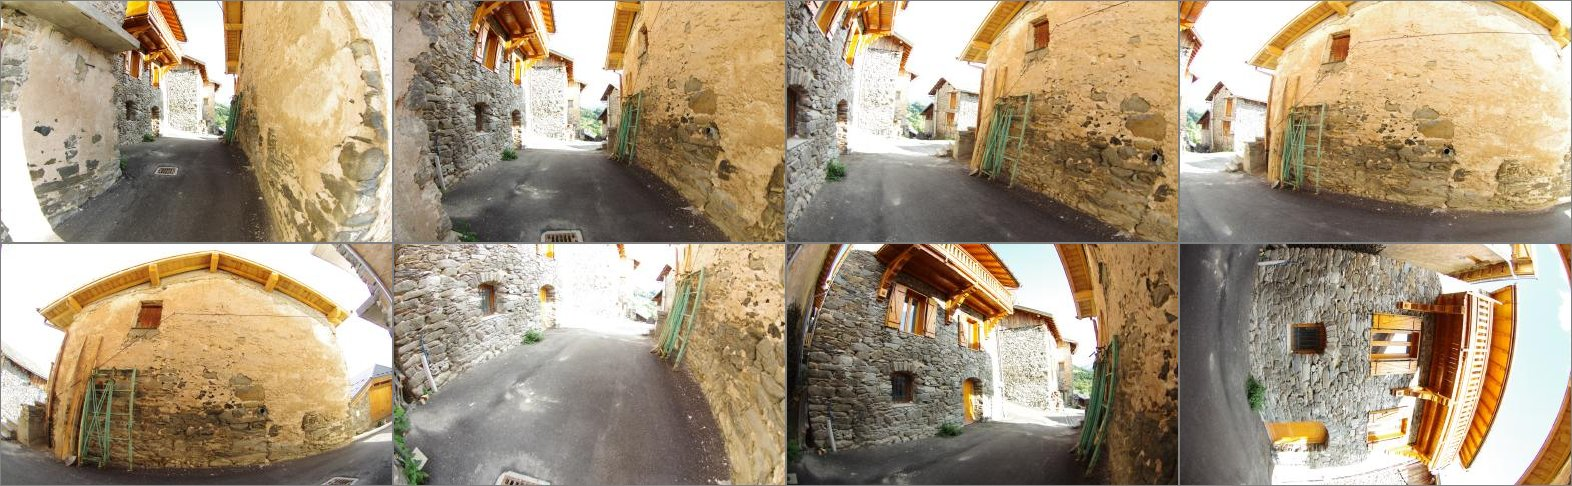
\includegraphics[width=150mm]{FIGS/StreetSainMartin/Planche-Rue.jpg}
\end{center}
\caption{Some of $10mm$-Saint martin's street photos}
\label{FIG:StM:Rue}
\end{figure}


\begin{figure}
\begin{center}
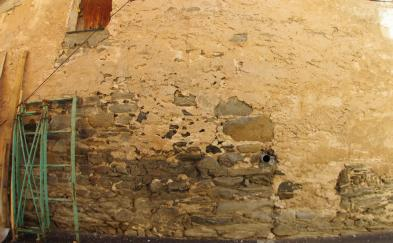
\includegraphics[width=30mm]{FIGS/StreetSainMartin/Small-IMGP4148.JPG}
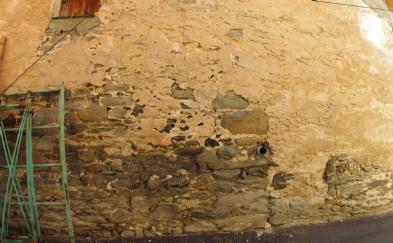
\includegraphics[width=30mm]{FIGS/StreetSainMartin/Small-IMGP4149.JPG}
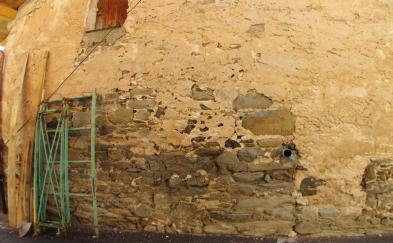
\includegraphics[width=30mm]{FIGS/StreetSainMartin/Small-IMGP4150.JPG}
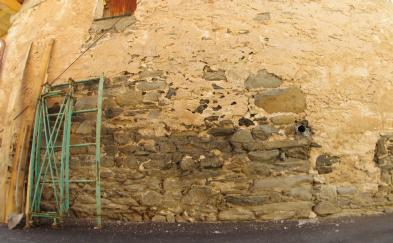
\includegraphics[width=30mm]{FIGS/StreetSainMartin/Small-IMGP4151.JPG}
\end{center}
\caption{One of the  $17mm$-Saint martin's street subset}
\label{FIG:StM:StrConv}
\end{figure}


To obtain the necessary tie points, one can type (you can find it
inside the file {\tt ExCmd.txt}) :


\begin{verbatim}
Tapioca All "IMGP41((1[8-9])|(2[0-2])).JPG" 1000
Tapioca All "IMGP41((5[2-8])).JPG" 1000
Tapioca All "IMGP41((2[3-9])|[3-4][0-9]|(5[0-1])).JPG" 1000
\end{verbatim}



\subsection{Exploiting the data with {\tt Tapas}}

To exploit the acquisition strategy described above, a pertinent processing
strategy will be also separated in several steps; for example:

\begin{itemize}
    \item  orientate at first the  short focal lenses, that will constitute the
           global canvas 
    \item  compute the orientations of other images based on the canvas of
            the already oriented images;
\end{itemize}

Using this general strategy , with the Saint Martin Street dataset,
we would like to proceed this way:

\begin{itemize}
    \item  compute the calibrations of the camera;
    \item  compute the orientations of the $10mm$ images only;
    \item  compute the orientations of the $17mm$ images,  in the same
           coordinate system that the already oriented  $10mm$ images;
\end{itemize}

The following commands could realize this program :


\begin{verbatim}
Tapas FishEyeEqui   "IMGP41((1[8-9])|(2[0-2])).JPG"  Out=Calib10
Tapas FishEyeEqui   "IMGP41((5[2-8])).JPG"  Out=Calib17

Tapas AutoCal   "IMGP41((2[3-9])|[3-4][0-9]|(5[0-1])).JPG"  InCal=Calib10 Focs=[9,11] Out=Tmp1

cp Ori-Calib17/AutoCal170.xml Ori-Tmp1/
Tapas FishEyeEqui   "IMGP41((2[3-9])|[3-4][0-9]|(5[0-1])).JPG"  InOri=Tmp1  Out=all

AperiCloud "IMGP41((2[3-9])|[3-4][0-9]|(5[0-1])).JPG" all
\end{verbatim}

Let's comment  :

\begin{itemize}
   \item  the fisrt two lines generates an initial calibration  with the calibration subsets;
          it is quite similar to~\ref{Succ:Call:Tapas}, the difference being that the 
          {\tt FishEyeEqui} specifies that we have a fisheye;

   \item  the third line uses the  {\tt InCal} options, already seen;  it also
          uses the option {\tt Focs=[9,11]}, the effect is   that only the images
          with a focal lense between $9mm$ and $11mm$ will be loaded; so here we orientate
          the $10mm$ subset;

   \item the line {\tt cp Ori\dots}, is necessary because we will need, on next call to Tapas,
         to have all our required input on the same directory {\tt Ori-Tmp1}

    \item in the next call to {\tt Tapas}, we specify {\tt InOri=Tmp1},  this has two effects :
         
\begin{itemize}
         \item  as before when files {\tt Ori-Tmp1/AutoCalXXX.xml} ( {\tt XXX} being the required focal) exist
                they are used to initialize intrinsic calibrations;

         \item  when files  {\tt Ori-Tmp1/OrientationXXX.xml} ({\tt XXX} being the images
                name) exist they are used to initialize the \UNCLEAR{external orientations};%intrinsic calibration
\end{itemize}
    \item  so here, we will stary directly from "good" initial value for both intrinsic calibration
           and external orientation of $10mm$ images.

\end{itemize}


%-------------------------------------------------------------------
%-------------------------------------------------------------------
%-------------------------------------------------------------------
\section{Camera data base and exif handling}

\subsection{How {\tt Tapas} initialize calibration}

For each camera it has to handle, when the user do not provide a calibration
file, {\tt Tapas} has to build an initial  value. For all parameters, but the
focal it's relatively easy :

\begin{itemize}
  \item for the distorsion , the initial value is nul \footnote{more
        precisely, it is the initial physical model, for example 
        with fish-eye the initial value is a $\tan^{-1} $ function, see~\ref{SpGeo:FishEye}};

  \item for the principal point the initial value is a at center of image 
        \footnote{ of course, this wouldnt  be suitable with shift lenses}.
\end{itemize}

For the focal lens Tapas must compute an initial value in pixel, this information is 
computed with the help of xif data. To see some example of xif data, goto MurSaint martin
and try {\tt ElDcraw -i -v} or {\tt exiv2} or {\tt exiftool} :

\begin{verbatim}
ElDcraw -i -v IMGP4182.JPG
...
Camera: PENTAX K-5
....
Focal length: 28.0 mm
Focal Equi35: 42.0 mm
....
\end{verbatim}

As the xif meta data never contains directly the focal in pixel , 
several case can  occur :

\begin{itemize}
  \item if the xif meta data contain the value $F_{35}$ of the focal in equivalent $35mm$  
       \footnote{try {\tt ElDcraw FileName} to see}, then the focal is estimated by
       $\frac{F_{35} * W_{Pix}}{35.0}$, where $W_{Pix}$ is the witdh (= number) 
       of image in pixel;

  \item if the xif meta data contain the value $F_{mm}$ of the focal in milimeter, 
        and the width  $W_{mm}$  of the sensor is known  in milimeter, the focal is estimated
        by $\frac{F_{mm} * W_{Pix}}{W_{mm}}$.

\end{itemize}

The size of the sensor is not a xif tag, so the information has to come from
somewhere else; this is the role of the camera data base.


\subsection{Camera data base}
\label{CamDB}

With all camera sold for people, xif meta data contain a tag indicating the 
name of the camera.  For example you can see that the {\tt MurSaintMartin }
has been acquired with a {\tt PENTAX K-5} camera. This camera name is
used by the different tools as an entry in data bases containing  informations
absent from xif files.

These data base can be located in three different files :

\begin{itemize}
   \item  {\tt  include/XML\_MicMac/DicoCamera.xml} , this global file always exist as
         it is part of the {\tt MicMac} distribution, I put here the camera necessary
         for the examples; I also update it when I  I meet a new camera 
         so that  users can take benefit of it;
         NEVER modify this file to add your own camera, as your may loose all your
         modification at next update; 
   
   \item  {\tt  include/XML\_User/DicoCamera.xml} , this file does not exist
         when you make the first instatllation of MicMac; so you have to create it,
         and put inside the descritption of all the camera that you will use
         currently; as this file is not handled by subversion, there is no risk
         of over writing it when you update;

   \item  {\tt  MicMac-LocalChantierDescripteur.xml},  in your working 
          directory when this file exists; the {\tt ENAC} example contains
          en example of such usage;
\end{itemize}

Naturally , if the same camera is described in several file, the more local file has the 
priority \footnote{e.q. {\tt MicMac-LocalChantierDescripteur.xml} highest priority
{\tt XML\_MicMac/DicoCamera.xml} lowest} .
Take a look at  {\tt  include/XML\_MicMac/DicoCamera.xml}, the structure is quite
simple :

\begin{itemize}
    \item a {\tt MMCameraDataBase} contains  a {\tt CameraEntry} for each  camera
          to describe;
    \item a {\tt CameraEntry} contains :

 
     \begin{itemize}
           \item a {\tt Name} that is used to make the link with information in xif file;
           \item a {\tt SzCaptMm} that contains the size of sensor in millimeter;
           \item a {\tt ShortName} which usage will be explained later  in~\ref{DB:Calib};
                (just give the value {\tt XXXX} until here)
     \end{itemize}
\end{itemize}


\subsection{Indicating missing xif info}

Sometimes, the xif file does not contain the expected information. This can be the
case for example when images where acquired by industrial camera, or when the images
result from conversion by various software. In this case, the information can be indicated "dynamically"
by creating specific key in the {\tt  MicMac-LocalChantierDescripteur.xml}.

The {\tt ENAC} dataset  illustrate this usage :

\begin{itemize}
    \item to indicate camera names, the user must define a rule 
           (see \ref{Ref:Key:Map}) of key  {\tt NKS-Assoc-STD-CAM}, this rule must
           transform the name of the file into the name of the camera;
           in {\tt ENAC} there is only one camera, the rule specify  then that,
           whatever be the image name, the camera name will be {\tt TheGOPRO};
 

    \item to indicate focal lenght, the user must define a rule 
          of key {\tt NKS-Assoc-STD-FOC} that associate to each image name
          its focal; here we have only one focal $3.8$, the rule is simple;


    \item the association mecanism desribed in \ref{Ref:Key:Map} may seem 
          over complicated, however it has to be very flexible to handle case
          where there are several cameras or focal lenghts not present in xif files;

\end{itemize}


\subsection{Modifying  exif}

Another solution to deal with missing xif info is to use the 
modifying facilities offered by the  exiv2 command .
I recommand that you read carrefully
the exiv2 documentation before using it. Here is a short example,
without  any warantee.

First create a commande file, let name it {\tt Cmd.txt} with the appropriate syntax :

\begin{verbatim}
set Exif.Photo.FocalLength 120/1
set Exif.Photo.FocalLengthIn35mmFilm 180
\end{verbatim}

Then execute this command file on the desired images by something like :

\begin{verbatim}
exiv2 -m"Cmd.txt"  *.PEF
\end{verbatim}

%-------------------------------------------------------------------
%-------------------------------------------------------------------
%-------------------------------------------------------------------

\section{Other options of Tapas}

\subsection{Saving intermediar results with {\tt SauvAutom}}

\subsection{Forcing first image with {\tt ImInit}}

\subsection{Freezing poses with  {\tt FrozenPoses}}

The optional arg {\tt FrozenPoses} of {\tt Tapas}, can be used to indicate
a subset of images for which orientation will be frozen during all the
compensation;  {\tt FrozenPoses} is a generalized regular expression  
(pattern or key) describing this subset.



%-------------------------------------------------------------------
%-------------------------------------------------------------------
%-------------------------------------------------------------------

\section{Other tools for orientation}


%-------------------------------------------------------------------

\subsection{The tool {\tt AperiCloud}}
\label{APERICLOUD}

This section describes {\tt AperiCloud} a simplified version of the
{\tt <ExportNuage>} section of {\tt Apero} described in~\ref{Ap:Exp:Nuage}.


For example with Mur Saint Martin:

\begin{verbatim}
AperiCloud "./IMGP41((6[7-9])|([7-8][0-9])).JPG" Mur
\end{verbatim}


Typing {\tt AperiCloud -help}, one gets:

\begin{verbatim}
*****************************
*  Help for Elise Arg main  *
*****************************
Unamed args : 
  * string
  * string
Named args : 
  * [Name=ExpTxt] INT
  * [Name=Out] string
  * [Name=Bin] INT
  * [Name=RGB] INT
\end{verbatim}

Meaning of args is:

\begin{itemize}
   \item First arg: pattern specifying the set of images ;
   \item Second  arg: pattern specifying the directory where orientations are located:
   \item optional {\tt ExpTxt}, def = $0$, set to $1$ if tie points are to be red in text format;
   \item optional {\tt Out}, def = AperiCloud.ply , specify the name of the generated ply file;
   \item optional {\tt Bin}, def = $1$ , set to  $0$  if ply file are to be generated in text format;
   \item optional {\tt RGB}, def = $1$ , set to  $0$  if the point are to be coloured with black
          and white images (usefull to save time);
\end{itemize}

%-------------------------------------------------------------------

\subsection{The tool {\tt Campari}}
\label{CAMPARI}

This section describes {\tt Campari} an interface to {\tt Apero}, for compensation 
of heterogenous measures, that is: tie points and ground control points.

\vspace{\baselineskip}
For example:

\begin{verbatim}
Campari "MyDir\IMG_.*.jpg" OriIn OriOut GCP=[GroundMeasures.xml,0.1,ImgMeasures.xml,0.5]
\end{verbatim}

Typing {\tt Campari -help}, one gets:

\begin{verbatim}
*****************************
*  Help for Elise Arg main  *
*****************************
Unamed args :
  * string :: {Full Directory (Dir+Pattern)}
  * string :: {Input Orientation}
  * string :: {Output Orientation}
Named args :
  * [Name=GCP] vector<std::string> :: {[GrMes.xml,GrUncertainty,ImMes.xml,ImUnc]
\end{verbatim}

Meaning of args is:

\begin{itemize}
   \item First arg: pattern specifying the set of images ;
   \item Second arg: pattern specifying the directory where orientations are located:
   \item Third arg: pattern specifying the directory where to write output orientations:
   \item optional {\tt GCP}, specifying the ground and image measures files, with their respective uncertainties;
\end{itemize}

\vspace{\baselineskip}
Mandatory part of GCP:
\begin{itemize}
\item xml file with 3D coordinates for GCP
\item GCP ground uncertainty
\item xml file with 2D coordinates for GCP
\item GCP image uncertainty
\end{itemize}

\vspace{\baselineskip}
The xml file containing 3D coordinates has to verify a specific format.
A tool to convert existing coordinates listing files into this format 
is proposed with {\tt GCPConvert} and described in \ref{GCPConvert}.

\vspace{\baselineskip}
The xml file containing 2D coordinates can be generated using interfaces 
{\tt SaisiePointsInit} and {\tt SaisiePointsPredic} in Linux, described in \ref{SaisieAppuisInit}.

\vspace{\baselineskip}
For a detailed example on how to use {\tt Campari} in a typical aerial 
surveying workflow, see \ref{Cuxa:DataSet}.

%-------------------------------------------------------------------
%-------------------------------------------------------------------
%-------------------------------------------------------------------

\section{The Bascule's tools}

\subsection{Generalities}

\label{BASCULE}
This section, describe the simplified version of the {\tt <BasculeOrientation>} mechanisms
described in~\ref{SC:Base:Or}. This mechanisms is used when global transformation of the 
orientation is required. The tools for bascule are :

\begin{itemize}

   \item {\tt SBGlobBascule}  is a tool for "scene based global" bascule,
         it is used when no absolute information is avalaible but the user
         still wishes to give some physicall meaning to the orientation;
         
   \item {\tt GCPBascule}  for using ground control point (GCP) to make
         a global transformation from a generally purely relative orientation
         to an orientation in the system of the GCP;

   \item {\tt RepLocBascule} a tool usefull to define a local repair without
         changing the orientation;

   \item {\tt EGSBascule}  for using embeded GPS on submit  to make
         a global transformation from a generally purely relative orientation
         to an absolute orientation : \emph{to come \dots}


   \item   the {\tt Bascule} used to do, more a less, all of the previous 
           functionnality; it is obsolete, still maintained for compatibility,
           but no longer documented;
\end{itemize}


        %  -    -    -    -    -    -    -     -
\subsubsection{Scene based orientation with {\tt SBGlobBascule}}

\label{ScBas:Basc}
 
A current case in architectural modeling, is when a part of the
scene is \emph{globally} plane and we want to do computation in
coordinate system where this plane is the horizontal plane. 
This can be done with the tool {\tt SBGlobBascule}:



\begin{itemize}
   \item {\tt SBGlobBascule} use a selected number of images, on which the
         user has created mask, these mask mut defined part of the image
         belonging to the plane (see figure~\ref{FIG:MaskPlane:StMartin} as an
         example);

   \item {\tt SBGlobBascule} select the tie points belonging to the mask, and
         compute by least square fitting an estimation of this  plane;


   \item finally bascule {\tt SBGlobBascule} compute the rotation that transform
         current coordinates in a new system where the fitted plane correspond to 
         the plane $Z=0$;

    \item {\tt SBGlobBascule}  fix  also the orientation inside the plane;

    \item optionnally {\tt SBGlobBascule}  can fix the  the global scale;
\end{itemize}


\begin{figure}[H]
\begin{center}
\includegraphics[width=50mm]{FIGS/MurSaintMartin/Plan1.jpg}
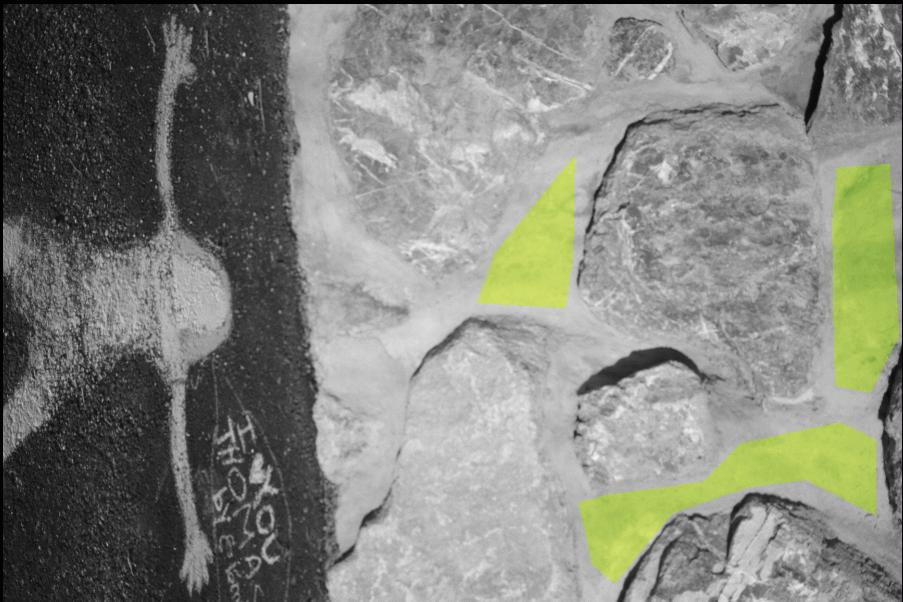
\includegraphics[width=50mm]{FIGS/MurSaintMartin/Plan2.jpg}
\end{center}
\caption{Example of masks defining a plane}
\label{FIG:MaskPlane:StMartin}
\end{figure}


With the dataset od street Saint Martin, an example of use is :

\begin{verbatim}
SBGlobBascule "IMGP41((6[7-9])|([7-8][0-9])).JPG" Mur MesureBasc.xml  LocBasc PostPlan=_MasqPlan  DistFS=0.6
\end{verbatim}

The meaning of the arguments are:

\begin{itemize}
  \item first arg, is the pattern defining the image we want to use;

  \item second arg {\tt Mur} defines the input orientation;

  \item third arg {\tt MesureBasc.xml} is a file that contains image measurement
        for defining orientation;

  \item fourth  arg {\tt Basc} defines the output orientation;

  \item optional args {\tt PostPlan=\_MasqPlan}  means that if image is {\tt IMGP4171.JPG} 
        (or {\tt IMGP4171.CR2} or \dots), then the associated mask {\tt IMGP4171\_MasqPlan.tif}

   \item  if there are several masks it will use all them for
         fitting the plane (which can be usefull with wide dataset when high accuracy  is required);
         of course if there are no exitsing mask an error will occur;
  
  \item optional args {\tt DistFS=0.6} is used to fix the scale;
\end{itemize}


Open the file {\tt MesureBasc.xml}, you will see that it contains measurement
of points in image. Although the syntax should be quite obvious, it is
described in section~\ref{GCP:Org}. To create a file like {\tt MesureBasc.xml}
user can of course do it with a text editor, alternatively he can, on Linux,
use the interactive tool {\tt SaisieBasc}  described in \ref{SaisieBasc}.
Once created, the following information will be looked for by  {\tt SBGlobBascule}
in this file:

\begin{itemize}
   \item measurement of points named {\tt Line1} and  {\tt Line2};
         they will fix orientation in the plane by imposing that line
           {\tt Line1-Line2} is parallel to $Ox$;

   \item these points need only to be measured in one image, as they are
         assumed  to be in the plane  computed on the masq; is they have been
         measured several time, a warning will occur;

   \item optional a point {\tt Origine} to fix the origin of the repair;

   \item optionally two point {\tt Ech1} and {\tt Ech2} to fix the scale,
         each point must be entered in two image, so that a $3d$ position
         can be computed; when {\tt DistFS} is entered, new coordinate system
         is computed with the constraint that the distant between the $3d$  
         position of  {\tt Ech1} and {\tt Ech2} is equal to {\tt DistFS} ;
         if {\tt DistFS} is entered and {\tt Ech1} and {\tt Ech2} do not
         exist in at least two images, an error occurs;
\end{itemize}

To have the full syntax, as usual:

\begin{verbatim}
   SBGlobBascule -help
*****************************
*  Help for Elise Arg main  *
*****************************
Unamed args : 
  * string :: {Full name (Dir+Pat)}
  * string :: {Orientaion in}
  * string :: {XML File of Images Measures}
  * string :: {Out : orientation }
Named args : 
  * [Name=ExpTxt] bool
  * [Name=PostPlan] string
  * [Name=DistFS] REAL :: {Distance between  Ech1 and Ech2 to fixe scale (if not given no scaling)}
  * [Name=Rep] string :: {Target repere (Def = ki, ie normal is vertical)}
\end{verbatim}

The {\tt Rep} is decsribed in section~\ref{SGB:Rep}.


        %  -    -    -    -    -    -    -     -
\subsubsection{Geo-referencing with {\tt GCPBascule}}

\label{Sec:GCPBascule}

In the Mur Saint Marin data set, you cand find two files:

\begin{itemize}
  \item {\tt Ground-Pts3D.xml} contains the definition of $3$D points, using
        the syntax detailled in ~\ref{GCP:Org};
  \item {\tt GroundMeasure.xml}  contains the $2$D measurement of these points
        in images,  using the syntax detailled in ~\ref{GCP:Org}.
\end{itemize}


The {\tt GCPBascule} command, allows to transform a purely relative orientation,
as  computed with  {\tt Tapas}, in an absolute one, as soon as there is at leat
$3$ GCP whose projection are known in at least $2$  image. Here for example:


\begin{verbatim}
GCPBascule   "IMGP41((6[7-9])|([7-8][0-9])).JPG" Mur Ground Ground-Pts3D.xml GroundMeasure.xml
\end{verbatim}

To know the syntax of {\tt GCPBascule} :
\begin{verbatim}
  GCPBascule  -help
*****************************
*  Help for Elise Arg main  *
*****************************
Unamed args : 
  * string :: {Full name (Dir+Pat)}
  * string :: {Orientaion in}
  * string :: {Orientation out}
  * string :: {File for Ground Control Points}
  * string :: {File for Image Measurements}
Named args : 
  * [Name=L1] bool :: {L1 minimisation vs L2; (Def=false)}
\end{verbatim}


The meaning should be quite obvious:

\begin{itemize}
  \item  first arg define the set of images, which you want to change orientation;
  \item  secong arg define the locatiion of input orientations (generally it will be purely relative
         orientation generated using {\tt Tapas} as described above);


  \item  third arg define the location of output orientation that will be generated by {\tt GCPBascule}

  \item fourth arg design the file containing the GCP and their $3d$ measures ;
  \item fifth arg design the file containing the image measurement of GCP;
  \item  optional arg {\tt L1} indicates if the transformation from relative to absolute
         must be done using $L_1$ or $L_2$ minimisation ( as currently the  measuremes 
         will have some redundancy).
\end{itemize}

Although it is generally difficult to analyse in detail the results of orientation
by inspecting the file, you can check rapidely that there is some coherence in the result.
For exemple if you type {\tt grep Centre Ori-Ground/*}, you get:


{\scriptsize
\begin{verbatim}
Ori-Ground/Orientation-IMGP4167.JPG.xml:               <Centre>5.2020...  1.4890...  2.1157...</Centre>
Ori-Ground/Orientation-IMGP4168.JPG.xml:               <Centre>5.2002...  0.7974...  2.1018...</Centre>
 ...
Ori-Ground/Orientation-IMGP4177.JPG.xml:               <Centre>4.1747... -3.4504...  2.1690...</Centre>
 ...
Ori-Ground/Orientation-IMGP4182.JPG.xml:               <Centre>3.7778... -6.1801...  2.2321...</Centre>
Ori-Ground/Orientation-IMGP4183.JPG.xml:               <Centre>3.6802... -6.6812...  2.2037...</Centre>
\end{verbatim}
}

So you can verify that in the ground repair, where $Z$ axis coincides with the vertical,
all the image centre are approximatively at the same height, which is quite coherent with
the acquisition I did.

        %  -    -    -    -    -    -    -     -
\subsubsection{Creating local repair with {\tt RepLocBascule}}

\label{Sec:RepLocBascule}

When {\tt MicMac} and derived tools are used in ground geometry, the
defaut convention is:

\begin{itemize}
   \item  for rectification, the images are  generated with $Z=Cste$ ;
   \item  for matching, the generated grid represents $Z=f(x,y)$ ;
\end{itemize}


These conventions are perfectly ok in aerial photogrammetry, 
the context  in which {\tt MicMac} was originally developped. However,
it won't work in architectural context, to make the orthophoto of a
vertical wall in some ground coordinate system where $Z$ axis  is vertical.
For example, suppose we want to use the rectification tool {\tt Tarama} (see~\ref{Sec:Tarama})
with the orientation {\tt Ground} defined, in~\ref{Sec:GCPBascule}.
If we type :

\begin{verbatim}
Tarama "IMGP41((6[7-9])|([7-8][0-9])).JPG" Ground Zoom=32
\end{verbatim}

Then we get the "rectified" image of figure ~\ref{FIG:PBRec:StMartin}. This
is probably not what we wanted.


\begin{figure}
\begin{center}
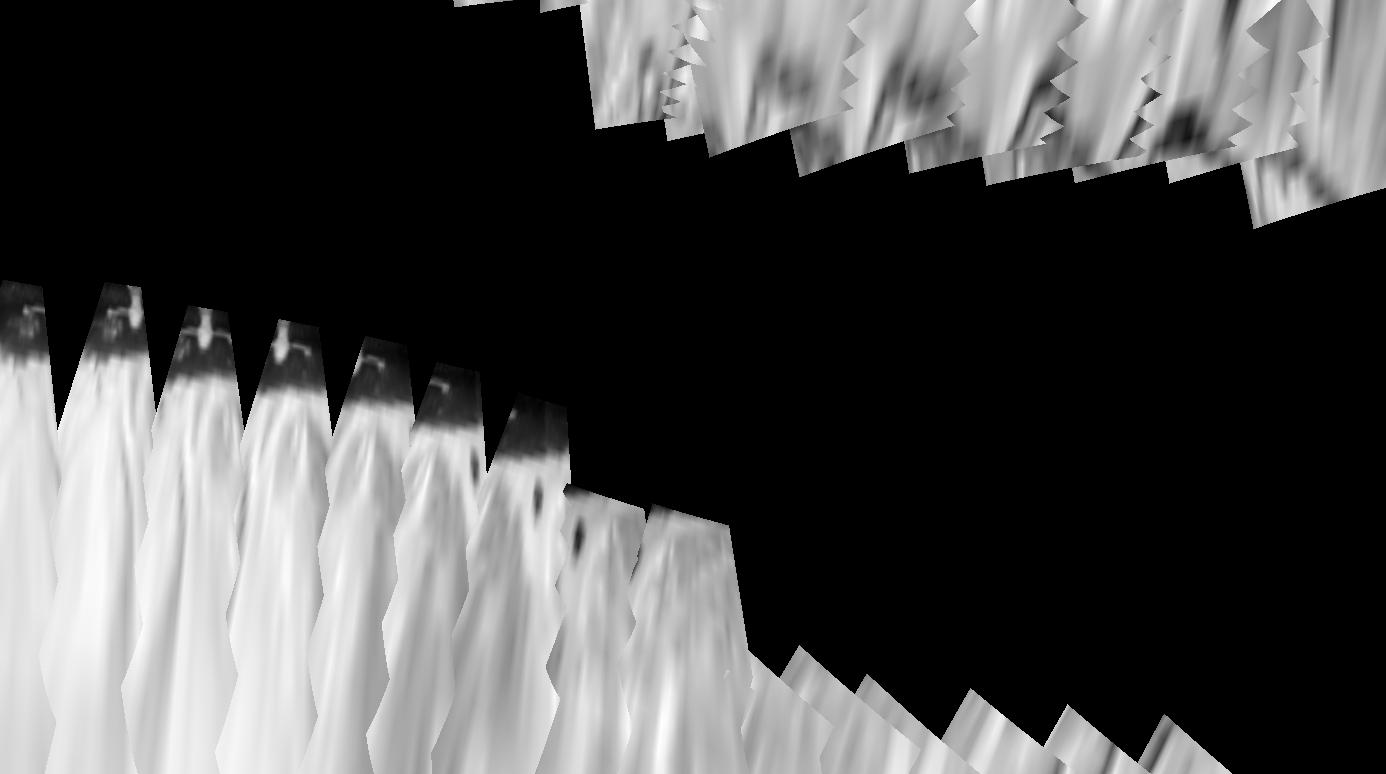
\includegraphics[width=120mm]{FIGS/MurSaintMartin/TA_PB_LeChantier.jpg}
\end{center}
\caption{Problem with Tarama applied directly in ground geometry}
\label{FIG:PBRec:StMartin}
\end{figure}

In such case, what we want to do is to define, for the matching, rectification \dots
purpose a \emph{local} repair with $Z$ axis orthogonal to the wall. These local repairs
will not be used to change the orientation (we want to maintain all the data in the
same ground coordinate system), but they will be used to specify, during matching
and rectification, a geometry adapted to the scene.
The command to define such repair is {\tt RepLocBascule}, the syntax is:

\begin{verbatim}
RepLocBascule -help
*****************************
*  Help for Elise Arg main  *
*****************************
Unamed args : 
  * string :: {Full name (Dir+Pat)}
  * string :: {Input Orientaion}
  * string :: {XML File of Images Measures}
  * string :: {Out Xml File to store the results"}
Named args : 
  * [Name=ExpTxt] bool :: {Are tie point in ascii mode ? (Def=false)}
  * [Name=PostPlan] string :: {Pots fix for plane name, (Def=_Masq)}
  * [Name=OrthoCyl] bool :: {Is the repere in ortho-cylindric mode ?}
\end{verbatim}

The meaning of the three first args is similar to {\tt SBGlobBascule}. The fourth 
arg specifies the output xml file.

In the data set of Mur Saint Martin, one could type:

\begin{verbatim}
RepLocBascule "IMGP41((6[7-9])|([7-8][0-9])).JPG" Ground MesureBasc.xml RepCorr.xml PostPlan=_MasqPlan
\end{verbatim}

The generated XML file {\tt RepCorr.xml} contains the necessary information to
describe a local repair: an origin and $3$ axis. Here:

\begin{verbatim}
<RepereLoc>
     <RepereCartesien>
          <Ori>-0.0303368933943062302 0.0014864175131534263 -0.0145221323781670186</Ori>
          <Ox>-0.00848394971784020499 0.99996077502067815 -0.00254381941768354975</Ox>
          <Oy>-0.00208480031723078411 0.00252621752215371033 0.99999463590194726</Oy>
          <Oz>0.999961837374218176 0.00848920756463100723 0.00206328623854717171</Oz>
     </RepereCartesien>
</RepereLoc>
\end{verbatim}

Next sections will describe how they can be used. The general principle is
simply to give these repair as optional argument to the program. For
example:

\begin{verbatim}
Tarama "IMGP41((6[7-9])|([7-8][0-9])).JPG" Ground  Repere=RepCorr.xml
\end{verbatim}

This will generate the rectified image of figure~\ref{FIG:OkRec:StMartin}.
 
\begin{figure}
\begin{center}
\includegraphics[width=120mm]{FIGS/MurSaintMartin/TA_OK-LeChantier.jpg}
\end{center}
\caption{Rectified image using the local repair}
\label{FIG:OkRec:StMartin}
\end{figure}


%-------------------------------------------------------------------

\subsection{MakeGrid}
\label{MAKEGRID}


%-------------------------------------------------------------------
%-------------------------------------------------------------------
%-------------------------------------------------------------------

\section{Tools for simplified matching}

\subsection{Basic rectification with {\tt Tarama}}

\label{Sec:Tarama}

To run the matching process (with {\tt MicMac} or {\tt Malt}) the
programm must decide which space has to be explored. If no
information is given, the programs will adopt a default strategy it
will select points of the scene that are visible on at least $N$ images
\footnote{generally $N=2$ or $N=3$}, 
making the assomption that the scene is globally flat. Althoug this
strategy may be perfectly ok on aerial acquisition, in the the general
case it may create a uselessly too large area. In general case, the
area selection requires some semantic interpretation of the scene
and can only me made by, you, the user who only knows what he wants.
For example, in the Saint Martin data set, an automatic program has no
information to determine that you want  to do the matching on the wall
and not on the street.

An easy way to indicate which part of the scene you want to use,
is to create a mask on a rectified mosaic.  The tool Tarama allows
to create such mosaic. At this step the relief is unkonw and the 
rectification is made with the assumption that $Z=ZMoy$, so of
course these mosaic are not very precise.

The syntax is:

\begin{verbatim}
 Tarama -help
*****************************
*  Help for Elise Arg main  *
*****************************
Unamed args : 
  * string :: {Full Imaeg (Dir+Pat)}
  * string :: {Orientation}
Named args : 
  * [Name=Zoom] INT :: {Resolution, (Def=8, must be pow of 2)}
  * [Name=Repere] string :: {local repair as created with RepLocBascule}
  * [Name=Out] string :: {drectory for output (Deg=TA)}
\end{verbatim}

The meaning of the two first mandotary arguments should be quite obvious now.
For the optional arguments:

\begin{itemize}
   \item  {\tt Zoom} indicates the resolution of the mosaic, it must be a power
          of $2$ as it is made using the image pyramid of {\tt MicMac};

   \item  {\tt Repere} indicates and optional repair created by {\tt RepLocBascule}
          as described in~\ref{Sec:RepLocBascule}
   \item {\tt Out} describes the directory where the mosaic will be created.
\end{itemize}

With the Mur Saint Martin data set,  using the orientation created with
{\tt SBGlobBascule} (\ref{ScBas:Basc}), one can type:

\begin{verbatim}
Tarama "IMGP41((6[7-9])|([7-8][0-9])).JPG" LocBasc
\end{verbatim}

The mosaic image will creatd on {\tt TA/TA\_LeChantier.tif}. 
Figure~\ref{FIG:Rectif:StMartin} shows the result.


\begin{figure}
\begin{center}
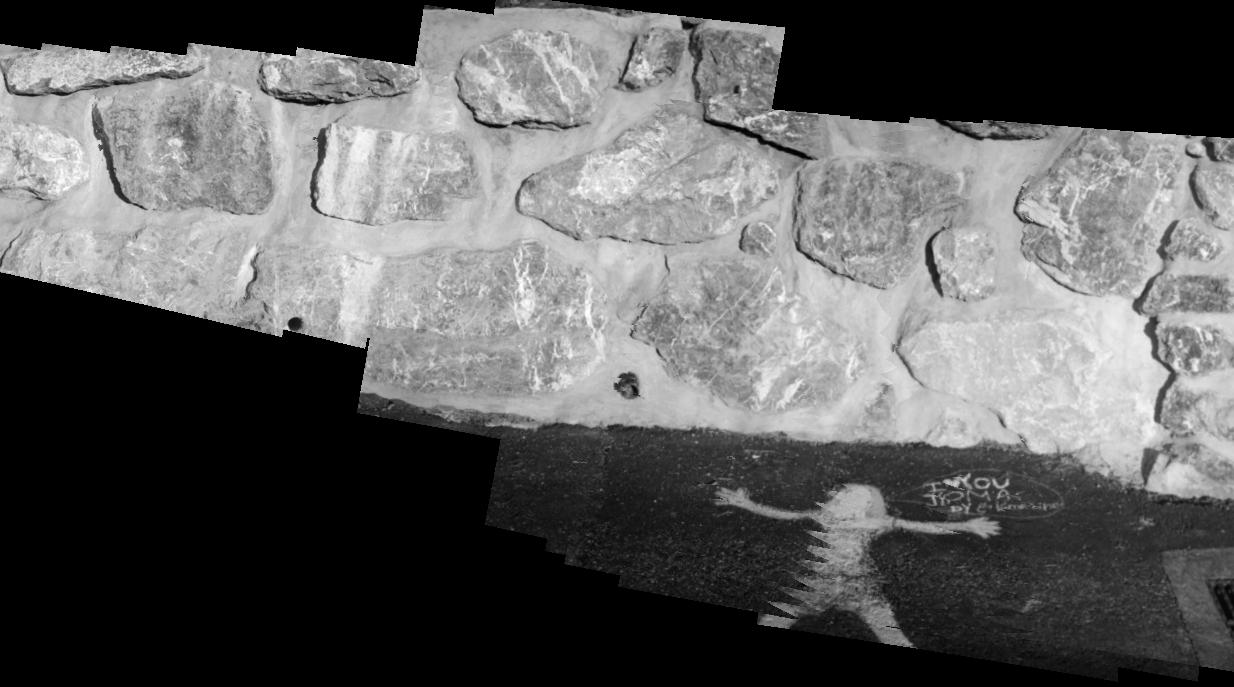
\includegraphics[width=120mm]{FIGS/MurSaintMartin/TA_LeChantier.jpg}
\end{center}
\caption{Result of Tarama of Mur Saint Martin data set}
\label{FIG:Rectif:StMartin}
\end{figure}


Example using local repair, have be done in~\ref{Sec:RepLocBascule}.



\subsection{Simplified matching in ground geometry with {\tt Malt}}

\subsubsection{General characteristics}

{\tt Malt} is a simplified  interface to  {\tt MicMac}. Currently it can
handle matching in ground geometry (see~\ref{Ground:Geom}) and 
ground-image geometry (see~\ref{EX:TER:IM:GEOM}).


Ground geometry is adapted
when the scene can be described by a single function $Z=f(X,Y)$ (with $X,Y,Z$
being euclidean coordinates); this case occurs quite often when the
scene is relatively flat and the acquisition is made by photo acquired 
orthogonaly to the main plane. The main use cases are:

\begin{itemize}
    \item  modelization of facades to generate ortho photo in architecture;
    \item  modelization of earth surface from aerial acquisition;
\end{itemize}

Ground image geometry is very general and flexible and can be used in
almost all acquisition. Its main drawbacks is that it requires~\footnote{for
now, I hope it will change in $2013$} some interaction to select the master images,
the mask of these images and  the associated secondary images.

The basic syntax requires $3$ args:

\begin{verbatim}
Malt Type Pattern Orient
\end{verbatim}

The meaning being:

\begin{itemize}
    \item  first args is a enumerated value, specifying the kind of matching required;
           the two possible values are:

     \begin{itemize}
          \item {\bf \tt Ortho} , for a matching adapted to ortho photo generation;
          \item {\bf \tt UrbanMNE} , for a matching adapted to urban digital elevation model;
          \item {\bf \tt GeomImage} , for a matching in ground image geometry;
     \end{itemize}


    \item  second arg specifies the subset of images;
    \item  third arg specifies the orientation;
\end{itemize}


An example with data set of Mur Saint Martin:


\begin{verbatim}
Malt Ortho "./IMGP41((6[7-9])|([7-8][0-9])).JPG" Basc
\end{verbatim}
  


A basic help can be asked with {\tt Malt -help}:

{\scriptsize
\begin{verbatim}
Malt -help
Valide Types for MNS : 
   Ortho
   UrbanMNE
   GeomImage
*****************************
*  Help for Elise Arg main  *
*****************************
Unamed args : 
  * string :: {Mode of correlation (must be in allowed enumerated values)}
  * string :: {Full Name (Dir+Pattern)}
  * string :: {Orientation}
Named args : 
  * [Name=Master] string :: { Master image must  exist iff Mode=GeomImage}
  * [Name=SzW] INT :: {Correlation Window Size (1 means 3x3)}
  * [Name=Regul] REAL :: {Regularization factor}
  * [Name=DirMEC] string :: {Subdirectory where the results will be stored}
  * [Name=DirOF] string
  * [Name=UseTA] INT :: {Use TA as Masq when it exists (Def is true)}
  * [Name=ZoomF] INT :: {Final zoom, (Def 2 in ortho,1 in MNE)}
  * [Name=ZoomI] INT :: {Initial Zoom, (Def depends on number of images)}
  * [Name=ZPas] REAL :: {Quantification step in equivalent pixel (def is 0.4)}
  * [Name=Exe] INT :: {Execute command (Def is true !!)}
  * [Name=Repere] string :: {Local system of coordinat}
  * [Name=NbVI] INT :: {Number of Visible Image required (Def = 3)}
  * [Name=HrOr] bool :: {Compute High Resolution Ortho}
  * [Name=LrOr] bool :: {Compute Low Resolution Ortho}
  * [Name=DirTA] string :: {Directory  of TA (for mask)}
  * [Name=Purge] bool :: {Purge the directory of Results before compute}
  * [Name=DoMEC] bool :: {Do the Matching}
  * [Name=UnAnam] bool :: {Compute the un-anamorphosed DTM and ortho (Def context dependant)}
  * [Name=2Ortho] bool :: {Do both anamorphosed ans un-anamorphosed ortho (when applyable) }
  * [Name=ZInc] REAL :: {Incertitude on Z (in proportion of average depth, def=0.3) }
  * [Name=DefCor] REAL :: {Default Correlation in un correlated pixels (Def = 0.2) }
  * [Name=CostTrans] REAL :: {Cost to change from correlation to uncorrelation (Def = 2.0) }
  * [Name=Etape0] INT :: {First Step (Def=1) }
  * [Name=AffineLast] bool :: {Affine Last Etape with Step Z/2 (Def=true) }
  * [Name=ResolOrtho] REAL :: {Resolution of ortho, relatively to images (Def=1.0; 0.5 mean smaller images) }
  * [Name=ImMNT] string :: {Filter to select images used for matching (Def All, usable with ortho) }
  * [Name=ImOrtho] string :: {Filter to select images used for ortho (Def All) }
  * [Name=ZMoy] REAL :: {Average value of Z}
  * [Name=Spherik] bool :: {If true the surface for redressing are spheres}
\end{verbatim}
}

For  optional parameters, the default value is generally dependant of the first
parameter. For example the parameter {\tt SzW}, defines the correlation
windows size, its default value is:


\begin{itemize}
   \item $1$ (ie window $3x3$) for DEM urban generation and ground image geometry
          because we want to preserve discontinuities;
   \item $2$ (ie window $5x5$) for ortho generation, because the priority here is robustness;
\end{itemize}

As usual these default values can be changed explicitly, for example:


\begin{verbatim}
Malt Ortho "./IMGP41((6[7-9])|([7-8][0-9])).JPG" Basc SzW=5
\end{verbatim}



\subsubsection{Optional parameters}

Table~\ref{Tab:ArgMalt} presents a summary of meaning and default value of
{\tt Malt} parameters;

\begin{figure}
\begin{tabular} { c | p{5 cm} | c | c | c}
{\bf Name }  &   {\bf Meaning } & {\bf Ortho } &  {\bf UrbanMNE} &{\bf GeomImage } \\  \hline \hline
{\bf SzW }  &   Sz correlation window & $2$ &  $ 1 $  &$1$ \\  \hline
{\bf Regul }  &  Regularization factor & $0.05$ &  $0.02$  & $0.02$ \\  \hline
{\bf UseTA }  &  Masq with TA & true &  true  & true \\  \hline
{\bf ZoomF }  &  Final resolution &  $2$ &  $1$   & $1$ \\  \hline
{\bf ZoomI }  &  Initial resolution &  XXX &  XXX   & XXX\\  \hline
{\bf ZPas }  &   Z quantification in pixel &  0.4 &  0.4  & 0.4 \\  \hline
{\bf Exe }  &   Execute the command &  true &  true   & true \\  \hline
{\bf Repere }  &   Name of a local repere for matching &  None &  None  & ?? \\  \hline
{\bf NbVI }  &   Minimal number of image visible in each ground point &  $3$ &  $3$ & $3$  \\  \hline
{\bf HrOr }  &   Compute High Resolution individual ortho photo &  true &  false  & ?? \\  \hline
{\bf LrOr }  &   Compute Low Resolution individual ortho photo &  true &  false  & ??\\  \hline
{\bf DirTA}  &   Directory where the mask is to search &  TA/ &  TA/   & ??? \\  \hline
\end{tabular}
\caption{Default values of malt parameters according to main options}
\label{Tab:ArgMalt}
\end{figure}

Some comments:

\begin{itemize}
   \item  the {\tt ZPas} does not specify directly a value in ground geometry;
         for a given value of a the {\tt ZPas} parameters,  {\tt MICMAC} will compute 
         the step, in ground geometry, such that, two consecutive projected point in images are 
         on average separated of {\tt ZPas};
         in the simple case where there would be two images, with a constant base-to-height ratio $R=\frac{B}{H}$,
         the step in ground geometry would be $\frac{ZPas}{R}$, 


   \item the {\tt NbVI}
\end{itemize}

\subsection{Image geometry with {\tt Malt}}

An example of using {\tt Malt} in mode {\tt GeomImage} 
with the {\tt Ramses} data set:

\begin{verbatim}
Malt GeomImage ".*CR2" All Master=IMG_0355.CR2
\end{verbatim}

There are some specificities when using {\tt Malt} in the mode {\tt GeomImage}:

\begin{itemize}
   \item  the parameter {\tt Master} must have a value, as it is the only way to
          distinguish the master image from the global set of image given by the pattern;
   \item the masq is not search in {\tt TA/TA\_LeChantier.tif}; if, for example, 
         the master  image is {\tt IMG\_0355.CR2} then the masq is {\tt IMG\_0355\_Masq.tif}
         for example
   \item the directory for storing results, depends from the master image, with {\tt IMG\_0355.CR2}
         it will be  {\tt MM-Malt-Img-IMG\_0355};
          
\end{itemize}


See~\ref{Analog:Image} for an example of using the {\tt Spherik} option.

%-------------------------------------------------------------------
%-------------------------------------------------------------------
%-------------------------------------------------------------------




%-------------------------------------------------------------------
%-------------------------------------------------------------------
%-------------------------------------------------------------------

\section{Ortho photo generation}

The simplified tool for generating ortho mosaic is {\tt Tawny}, it is
an interface to the {\tt Porto} tool described in~\ref{Porto}. 
The use of {\tt Tawny} is quite simple because it assumes that
the data have been correctly prepared and organized during the matching
process. Practically this is done when the macthing has been made using 
{\tt Malt} and I recommand to only use {\tt Tawny}  in conjonction with
{\tt Malt}. In Ortho Mode, {\tt Malt} has created a set of
individual ortho images, associated mask, incidence image, \dots in
a directory {\tt Ortho-MEC-Malt/}; see for example~\ref{FIG:Malt:Input}. 
 The job of {\tt Tawny} is essentially to merge these data and to optionnaly do some
radiometric equalization.



\begin{figure}
\begin{center}
\includegraphics[width=60mm]{FIGS/MurSaintMartin/Ort_IMGP4182.jpg}
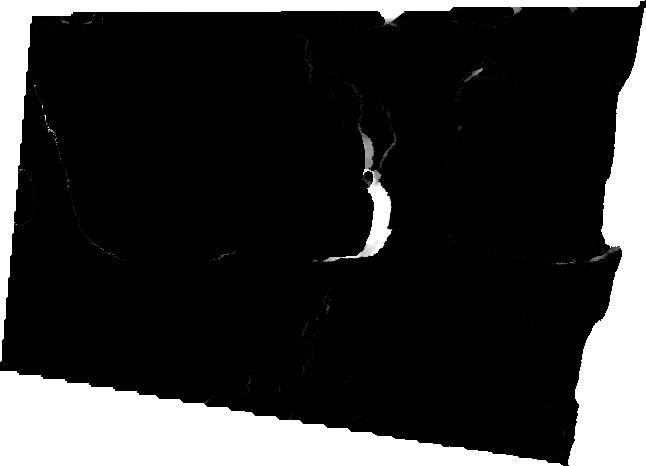
\includegraphics[width=60mm]{FIGS/MurSaintMartin/PC_IMGP4182.jpg}
\end{center}
\caption{Individual ortho image, and mask image for image {\tt IMGP4182.jpg}}
\label{FIG:Malt:Input}
\end{figure}

For the radiometric equalization, {\tt Tawny}  will compute for each
individual ortho image $O_i$, a polynom $P_i$ such that, $\forall i,j,x,y$
where ortho image $O_i$ and $O_j$ are both defined in $x,y$ we have the relation:

\begin{equation}
   O_i(x,y) P_i(x,y) = O_j(x,y) P_j(x,y)
\label{Eq:Rad:PolIndiv}
\end{equation}


The problem with such formula is that it can lead to important drift in radiometry.
So there is also a global polynom $R$ that is computed, this polynom is such that:

\begin{equation}
   O_i(x,y) P_i(x,y) R(x,y) =  O_i(x,y)
\label{Eq:Rad:PolGlob}
\end{equation}

The radiometry of each image used for the otho photo will finally be $O_i(x,y) P_i(x,y) R(x,y)$.
Of course for equation~\ref{Eq:Rad:PolIndiv} and~\ref{Eq:Rad:PolGlob}, there is
much more observations than unknowns and they are solved using least mean square.
The user can control the radiometric equalization by specifying the 
degree of the polynom. The syntax is:




\begin{verbatim}
Tawny -help
*****************************
*  Help for Elise Arg main  *
*****************************
Unamed args : 
  * string :: {Directory where are the datas}
Named args : 
  * [Name=DEq] INT :: {Degree of equalization (Def=1)}
  * [Name=DEq] INT :: {Degree of equalization (Def=1)}
  * [Name=DEqXY] Pt2di :: {Degree of equalization, if diff in X and Y}
  * [Name=AddCste] bool :: {Add unknown constant for equalization (Def=false)}
  * [Name=DegRap] INT :: {Degree of rappel to initial values, Def = 0}
  * [Name=DegRapXY] Pt2di :: {Degree of rappel to initial values, Def = 0}
  * [Name=RGP] bool :: {Rappel glob on physycally equalized, Def = true}
  * [Name=DynG] REAL :: {Global Dynamic (to correcyt saturation problems)}
  * [Name=ImPrio] string :: {Pattern of image with high prio, def=.*}
  * [Name=SzV] INT :: {Sz of Window for equalisation (Def=1, means 3x3)}
  * [Name=CorThr] REAL :: {Threshold of correlation to validate homologous}
  * [Name=NbPerIm] REAL :: {Average number of point per image}
\end{verbatim}

The only mandatory argument is the directory where the 
elementary ortho images have been created by {\tt Malt}. The parameters
{\tt DEq, DEqXY, AddCste, DegRap, DegRapXY} are relative to the correction
function used in radiometric equalization process:

\begin{itemize}
  \item {\tt DEq} specifies the degree of polynoms $O_i$, the default value is
        $1$ , which means that for each ortho image, $A_i,B_i,C_i$ are computed
        to satisfy according to least mean square the equation~\ref{Eq:Rad:Mon};

   \item {\tt DEqXY} specifies the case where the degree of $O_i$ are different in
         $x$ and $y$, if  {\tt DEqXY=[$D_X$,$D_Y$]}, the unknown monoms will
         be $x^n,y^m$ such that $n\leq D_X$ , $m\leq D_Y$ ,   $n+m\leq Max(D_X,D_Y)$;

   \item {\tt AddCste} in this case an unknown constant $K_i$ is add to each ortho $O_i$ and
          the equation ~\ref{Eq:Rad:PolIndiv} is replaced by ~\ref{Eq:Rad:PolIndivCste};
          in almost every case, it is preferable to let the default value {\tt AddCste=false};

   \item {\tt DegRap} fix the degree of global polynom $R$;

   \item {\tt DegRapXY} fix the degree of global polynom $R$ when different in $x$ and $y$;
    
\end{itemize}



\begin{equation}
O_i(x,y)(A_i+B_ix+C_iy)=O_j(x,y)(A_j+B_jx+C_jy);
\label{Eq:Rad:Mon}
\end{equation}

\begin{equation}
   O_i(x,y) P_i(x,y) + K_i = O_j(x,y) P_j(x,y) + K_j
\label{Eq:Rad:PolIndivCste}
\end{equation}

The table~\ref{Tab:Ortho:Polyn} illustrate the influence of this parameter:

\begin{itemize}
   \item first line, with the minimum degree parameter, {\tt DEq=0 DegRap=0} some
         frontier are visible;
   \item second line, with the default parameter, {\tt DEq=1 DegRap=0}, the frontier
         are almost not visible but there is clearly a drift in radiometry;
   \item third line line, with  degree $1$ polynom per image and a degre $2$ global
         attachement, the frontier are almost not visible and the drift has decreased:
   \item third line line, with  degree $1$ polynom per image and a degre $4$, the
         has disappeared except at points close to the border;
\end{itemize}

Note however that this data-set is surprisingly difficult to equalize for such a
small set. With many data sets, the default parameters already give an acceptable result.

% 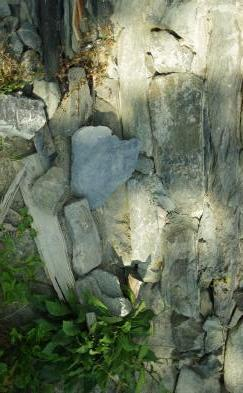
\includegraphics[width=25mm]{FIGS/MurSaintMartin/Small-IMGP4160.JPG}
\begin{figure}
\begin{tabular} { | c | p{2 cm} |  } \hline
 Images   &    Args opt  \\  \hline \hline
\includegraphics[width=150mm]{FIGS/MurSaintMartin/Ortho-Eg-Test-Redr-0-0.jpg}  &    DEq=0 \\  \hline 
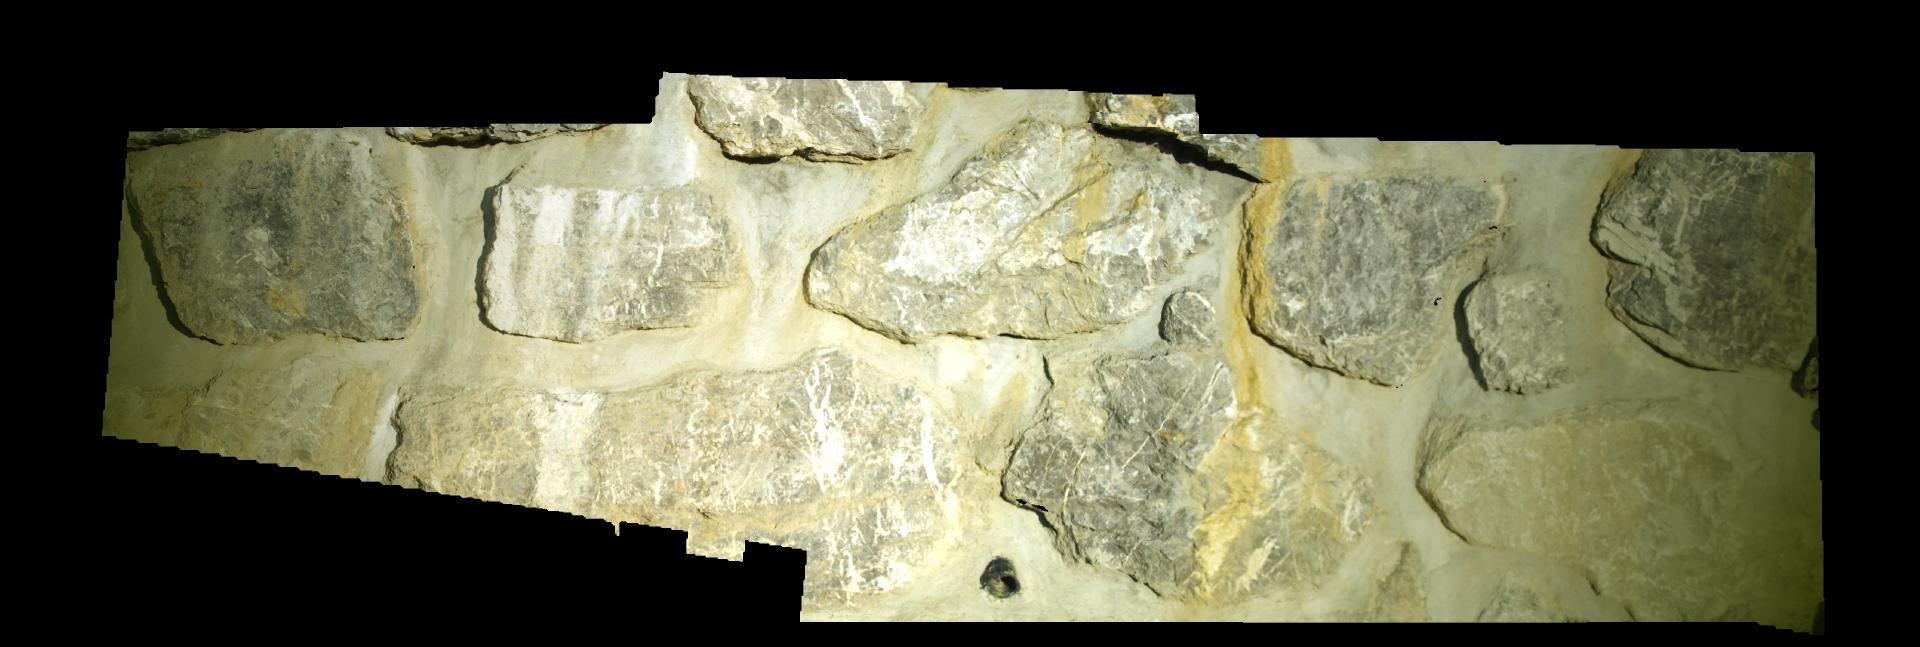
\includegraphics[width=150mm]{FIGS/MurSaintMartin/Ortho-Eg-Test-Redr-1-0.jpg}  &      \\  \hline 
\includegraphics[width=150mm]{FIGS/MurSaintMartin/Ortho-Eg-Test-Redr-1-2.jpg}  &    DEq=1 DegRapXY=[2,0] \\  \hline 
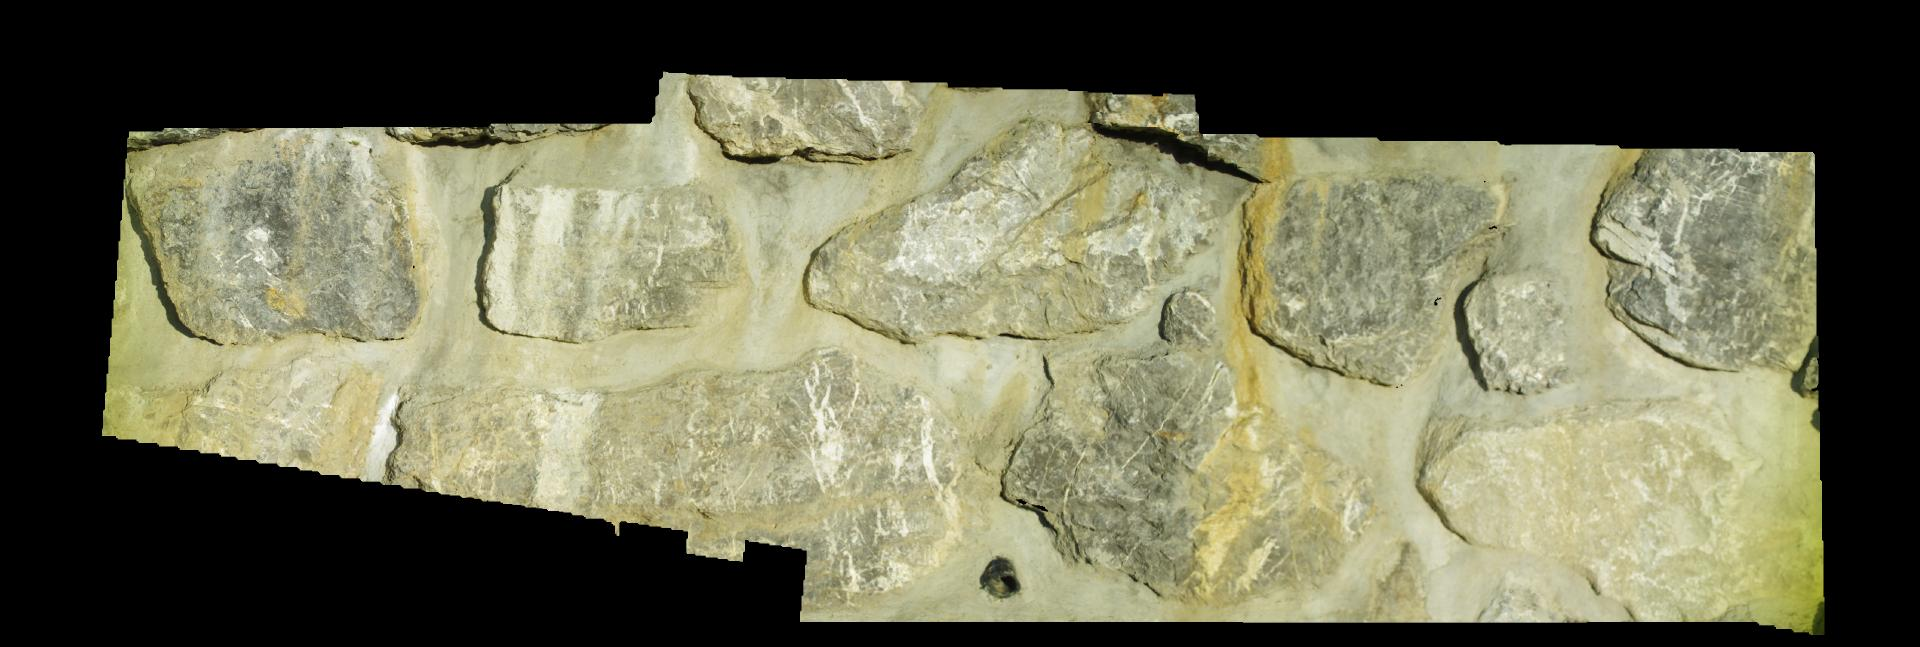
\includegraphics[width=150mm]{FIGS/MurSaintMartin/Ortho-Eg-Test-Redr-1-4_1.jpg}  &    DEq=1 DegRapXY=[4,1] \\  \hline 
\end{tabular}
\caption{Exemple of influence of polynomial degre parameter on ortho equalization}
\label{Tab:Ortho:Polyn}
\end{figure}


The parameters {\tt SzV, CorThr, NbPerIm} are relative to the choice of the point
used for the radiometric equalization:


\begin{itemize}
   \item {\tt SzV} is the size of the patch used for each sample of the radiometric equalization,
         this patches will be used for computing an average valure and for correlation  \dots

   \item  \dots on each patch, correlation coefficient  $C{i,j}$ are computed between pair 
          of images, they are used only if  $C{i,j} > CorThr$ ;
 
   \item {\tt NbPerIm} indicates the number of sample that will be approximatively used on each image;

\end{itemize}


On many data sets the default values should be OK. However it happened with difficult data
sets that all the measures were refused for some images pair, which obviously led to an error.
Here is an example of the command I used on a data set with such difficulties:


\begin{verbatim}
Tawny Ortho-MEC-Malt/ DEq=1 DegRap=1 ImPrio=Ort_IMG_.* SzV=3 CorThr=0.6 NbPerIm=5e4
\end{verbatim}

